\subsection{Parameter Evolution} \label{Sec: Parameter Evolution}
In this section, we discuss the parameter evolution of the Saunders and Schechter luminosity function fits in figure \ref{Fig: Bolometric IR LF}. The evolution of $\phi^{*}$ and $L^{*}$ across redshift is presented in figure \ref{Fig: Param Evo} with values and $1\sigma$ errors in tables \ref{Tab: Param Evo ZF}, \ref{Tab: Param Evo AGN}, and \ref{Tab: Param Evo SF}. The best fitting parameter values were calculated using \texttt{scipy.optimize.curve\_fit} \citep{virtanen_scipy_2020} and 1$\sigma$ parameter uncertainties are calculated using \texttt{np.sqrt(np.diag(pcov))} \citep{harris_array_2020} which relates the covariance of the best-fit parameters. As discussed in section \ref{Sec: Bolometric IR LF}, our final redshift bin likely suffers from incompleteness. However, ZFOURGE's ability to probe fainter luminosities becomes advantageous at higher redshifts, providing more reliable constraints on the LF parameters. In our lowest redshift bins, where ZFOURGE is less effective, more pronounced $1\sigma$ errors are recorded.

To better constrain the faint end slope of the ZFOURGE total LF, we fix $\alpha=1.3$ across all redshift bins. This result differs from the literature where \cite{rodighiero_mid-_2010, gruppioni_herschel_2013} fix $\alpha=1.2$ whereas \cite{fu_decomposing_2010} leaves $\alpha$ as a free fitting parameter found to be $\alpha=1.46$ (respective to our Saunders fitting function). As we lack luminosity bins along the bright end of the LF, we fix the bright end $\sigma$ to values that fit best to the available literature. The CIGALE SF LF fits with a Schechter function and a faint end slope of $\alpha=1.2$, reflecting its shallower rise compared to the ZFOURGE total LF. Similarly, we use a Saunders function to fit the CIGALE AGN LF using $\alpha$ = 1.2. The faint end slopes of CIGALE LFs agree with the literature. Due to the absence of bright-end AGN luminosity bins, we incorporate data from \cite{thorne_deep_2022} to help constrain the fitting process.

\begin{figure}[h]
    \centering
    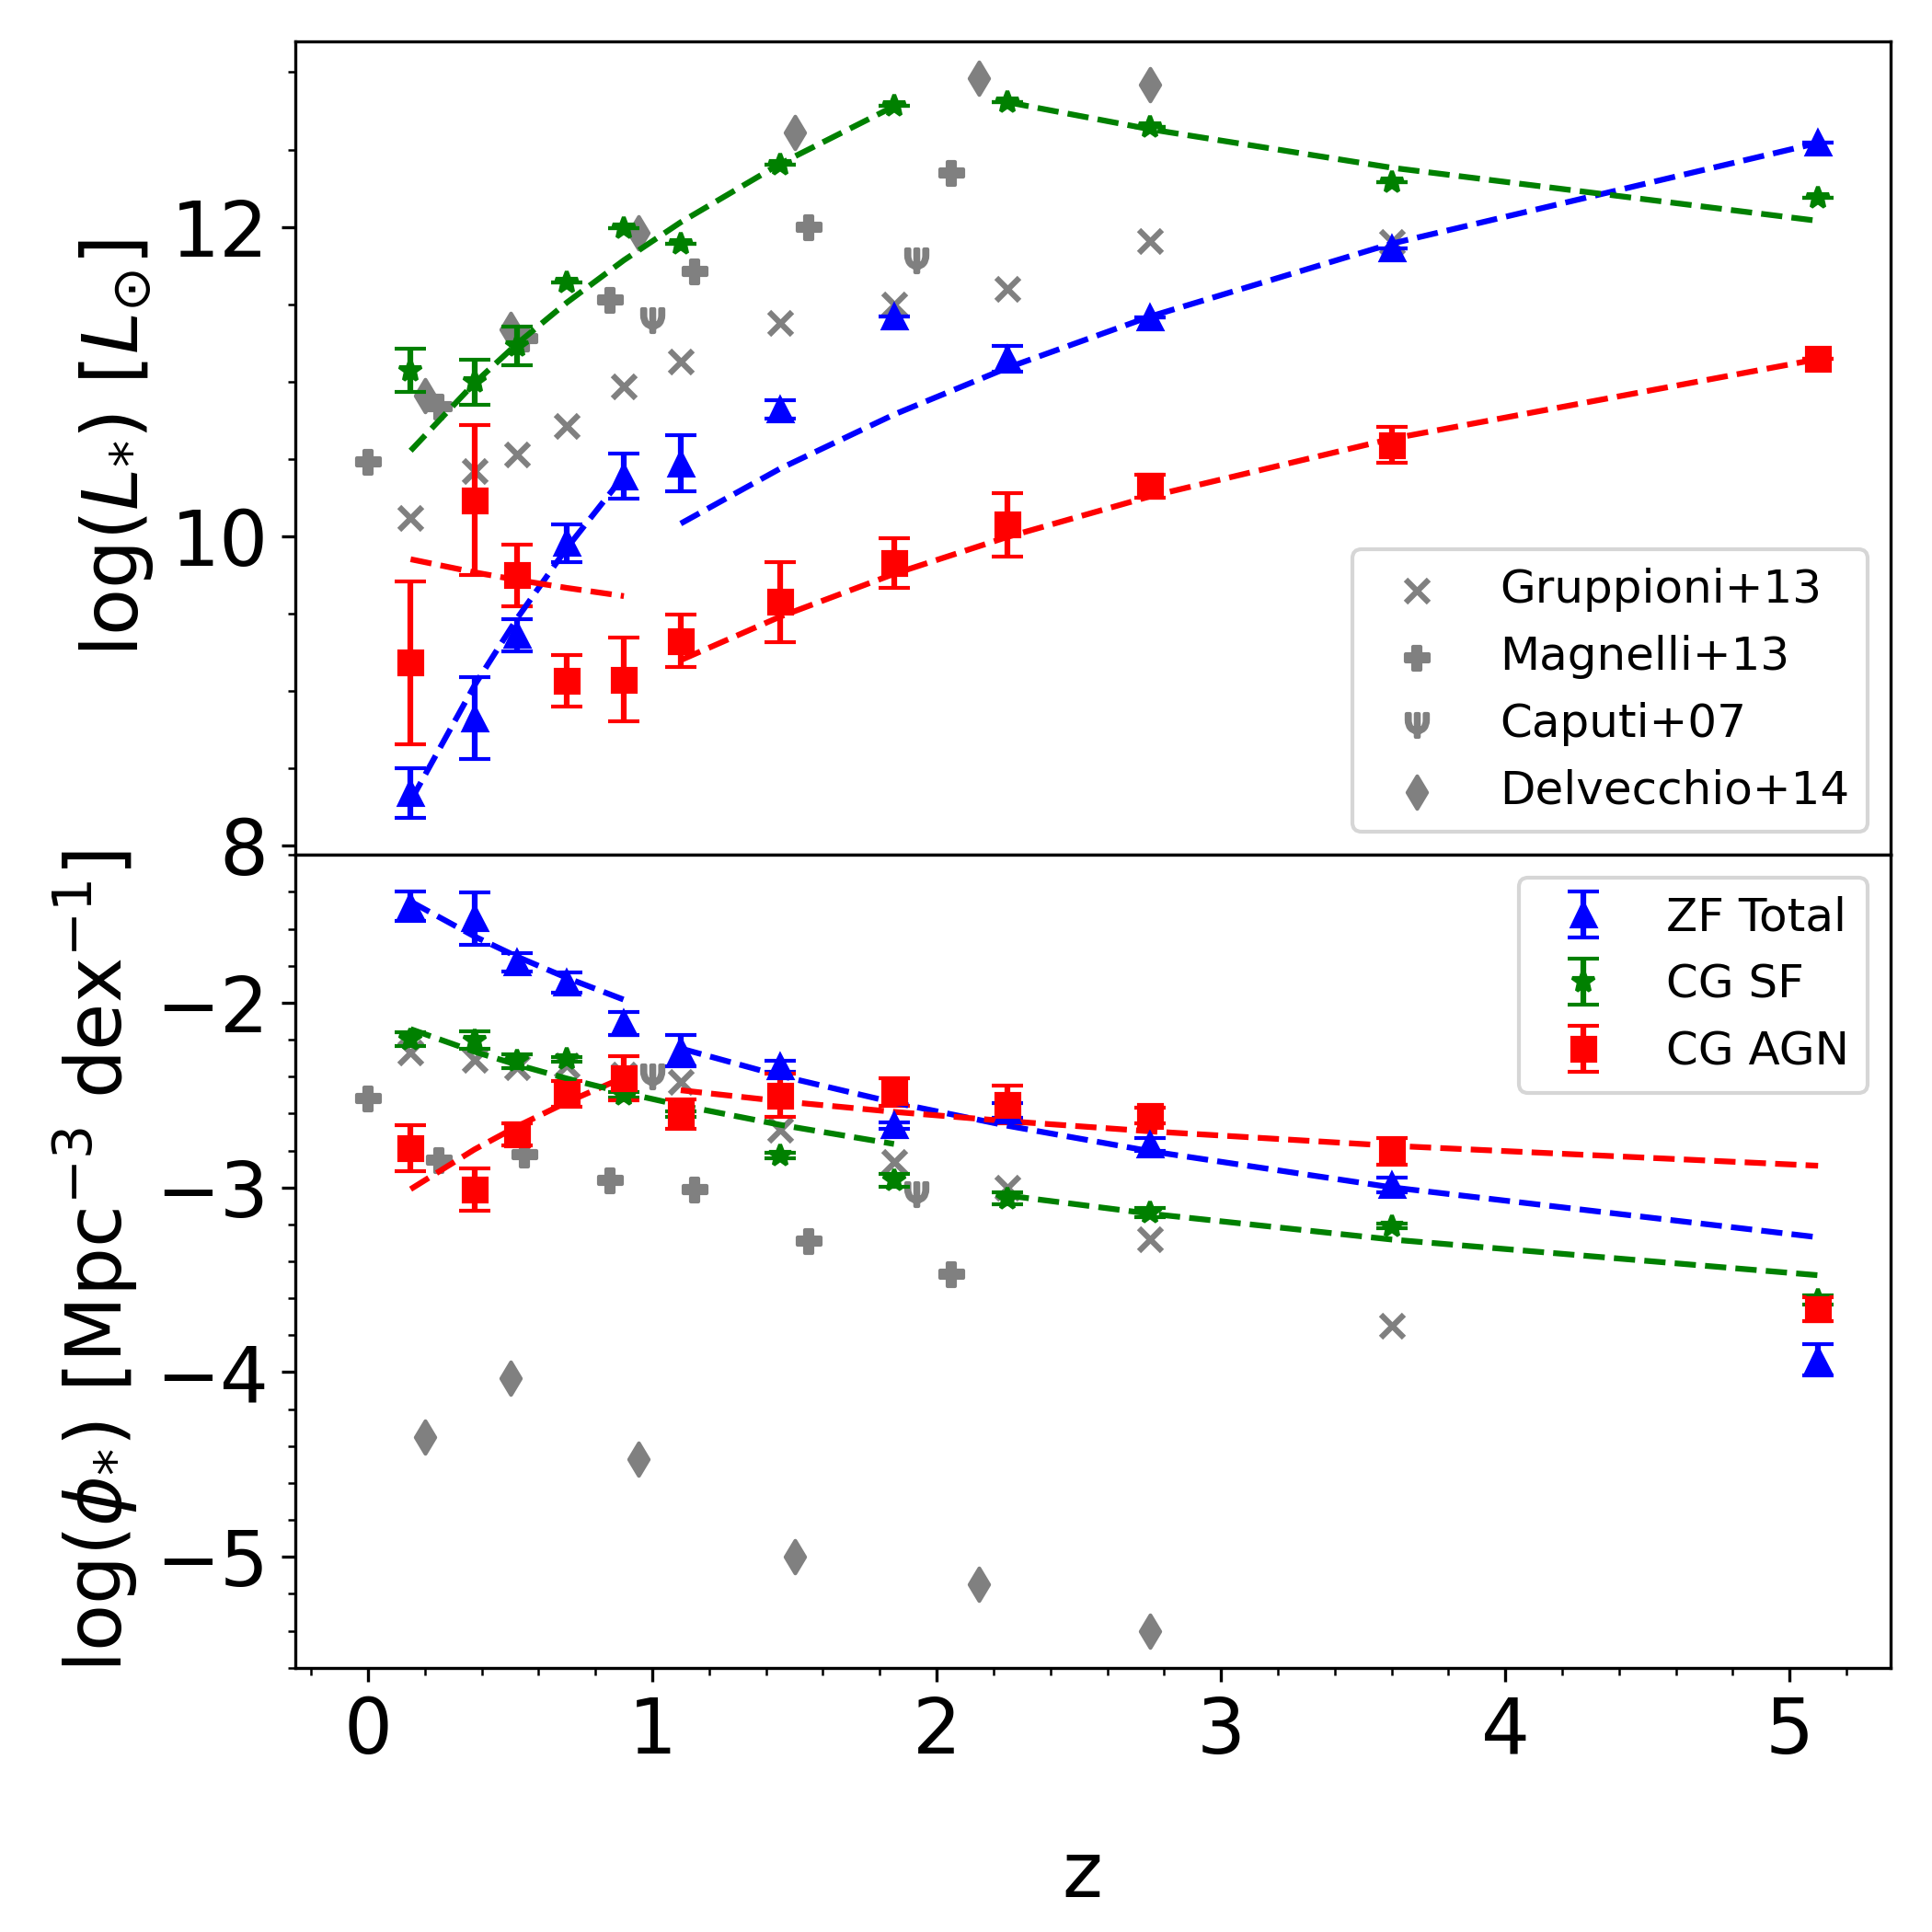
\includegraphics[width=0.48\textwidth]{Figures/Param Evo.png}
    \caption{Best fitting parameters and $1\sigma$ uncertainties to our luminosity functions. Top: $L^{*}$ evolution. Bottom: $\phi^{*}$ evolution. Blue triangles represent the ZFOURGE total. Red squares represent the CIGALE AGN and green crosses the CIGALE SF population. Dashed lines represent the $\propto(1+z)^k$ evolution. We compare our results to the relevant literature, which is coloured grey. \cite{gruppioni_herschel_2013} crosses, \cite{magnelli_deepest_2013} pluses, and \cite{caputi_infrared_2007} uppercase $\Psi$'s.}
    \label{Fig: Param Evo}
\end{figure}

\begin{table}[h]
    \caption{Best-fit parameters ($\log(L^*)$, $\log(\phi^*)$), along with fixed parameters ($\alpha, \sigma$), for the ZFOURGE total Saunders luminosity function across different redshift bins.}
    \label{Tab: Param Evo ZF}
    \begin{center}
    \begin{tabular}{ccccc}
        \toprule
        $z$ & log$(L^{*})$ & log$(\phi^{*})$ & $\alpha$ & $\sigma$ \\
        \hline
        0.00 $\leq z <$ 0.30 &  8.34 $\pm$ 0.16 & -1.48 $\pm$ 0.08 & 1.3 & 1.1 \\
        0.30 $\leq z <$ 0.45 &  8.82 $\pm$ 0.26 & -1.54 $\pm$ 0.14 & 1.3 & 1.0 \\
        0.45 $\leq z <$ 0.60 &  9.36 $\pm$ 0.10 & -1.78 $\pm$ 0.05 & 1.3 & 0.9 \\
        0.60 $\leq z <$ 0.80 &  9.96 $\pm$ 0.12 & -1.89 $\pm$ 0.05 & 1.3 & 0.8 \\
        0.80 $\leq z <$ 1.00 & 10.39 $\pm$ 0.14 & -2.11 $\pm$ 0.06 & 1.3 & 0.7 \\
        1.00 $\leq z <$ 1.20 & 10.47 $\pm$ 0.18 & -2.26 $\pm$ 0.09 & 1.3 & 0.7 \\
        1.20 $\leq z <$ 1.70 & 10.82 $\pm$ 0.06 & -2.35 $\pm$ 0.03 & 1.3 & 0.7 \\
        1.70 $\leq z <$ 2.00 & 11.42 $\pm$ 0.00 & -2.67 $\pm$ 0.02 & 1.3 & 0.7 \\
        2.00 $\leq z <$ 2.50 & 11.14 $\pm$ 0.08 & -2.58 $\pm$ 0.04 & 1.3 & 0.7 \\
        2.50 $\leq z <$ 3.00 & 11.42 $\pm$ 0.00 & -2.77 $\pm$ 0.03 & 1.3 & 0.7 \\
        3.00 $\leq z <$ 4.20 & 11.86 $\pm$ 0.00 & -2.99 $\pm$ 0.04 & 1.3 & 0.7 \\
        4.20 $\leq z <$ 6.00 & 12.54 $\pm$ 0.00 & -3.93 $\pm$ 0.08 & 1.3 & 0.7      
        \botrule
    \end{tabular}
    \end{center}
\end{table}

\begin{table}[h]
    \caption{Best-fit parameters ($\log(L^*)$, $\log(\phi^*)$), along with fixed parameters ($\alpha, \sigma$), for the CIGALE AGN Saunders luminosity function across different redshift bins.}
    \label{Tab: Param Evo AGN}
    \begin{center}
    \begin{tabular}{ccccc}
        \toprule
        $z$ & log$(L^{*})$ & log$(\phi^{*})$ & $\alpha$ & $\sigma$ \\
        \hline
        0.00 $\leq z <$ 0.30 &  9.19 $\pm$ 0.53 & -2.79 $\pm$ 0.13 & 1.2 & 1.0 \\
        0.30 $\leq z <$ 0.45 &  9.99 $\pm$ 0.59 & -2.96 $\pm$ 0.14 & 1.2 & 1.0 \\
        0.45 $\leq z <$ 0.60 &  9.42 $\pm$ 0.26 & -2.65 $\pm$ 0.08 & 1.2 & 1.0 \\
        0.60 $\leq z <$ 0.80 &  9.07 $\pm$ 0.17 & -2.49 $\pm$ 0.07 & 1.2 & 1.0 \\
        0.80 $\leq z <$ 1.00 &  9.07 $\pm$ 0.27 & -2.41 $\pm$ 0.12 & 1.2 & 1.0 \\
        1.00 $\leq z <$ 1.20 &  9.32 $\pm$ 0.17 & -2.60 $\pm$ 0.08 & 1.2 & 1.0 \\
        1.20 $\leq z <$ 1.70 &  9.57 $\pm$ 0.26 & -2.50 $\pm$ 0.12 & 1.2 & 1.0 \\
        1.70 $\leq z <$ 2.00 &  9.82 $\pm$ 0.16 & -2.49 $\pm$ 0.07 & 1.2 & 1.0 \\
        2.00 $\leq z <$ 2.50 & 10.07 $\pm$ 0.20 & -2.55 $\pm$ 0.10 & 1.2 & 0.9 \\
        2.50 $\leq z <$ 3.00 & 10.32 $\pm$ 0.07 & -2.61 $\pm$ 0.04 & 1.2 & 0.8 \\
        3.00 $\leq z <$ 4.20 & 10.59 $\pm$ 0.12 & -2.81 $\pm$ 0.07 & 1.2 & 0.7 \\
        4.20 $\leq z <$ 6.00 & 11.15 $\pm$ 0.00 & -3.66 $\pm$ 0.07 & 1.2 & 0.6      
        \botrule
    \end{tabular}
    \end{center}
\end{table}

\begin{table}[h]
    \caption{Best-fit parameters ($\log(L^*)$, $\log(\phi^*)$), along with fixed parameter ($\alpha$), for the CIGALE SF Schechter luminosity function across different redshift bins.}
    \label{Tab: Param Evo SF}
    \begin{center}
    \begin{tabular}{cccc}
        \toprule
        $z$ & log$(L^{*})$ & log$(\phi^{*})$ & $\alpha$ \\
        \hline
        0.00 $\leq z <$ 0.30 & 11.07 $\pm$ 0.14 & -2.20 $\pm$ 0.04 & 1.2 \\
        0.30 $\leq z <$ 0.45 & 11.00 $\pm$ 0.15 & -2.20 $\pm$ 0.05 & 1.2 \\
        0.45 $\leq z <$ 0.60 & 11.23 $\pm$ 0.12 & -2.32 $\pm$ 0.04 & 1.2 \\
        0.60 $\leq z <$ 0.80 & 11.64 $\pm$ 0.00 & -2.31 $\pm$ 0.01 & 1.2 \\
        0.80 $\leq z <$ 1.00 & 11.99 $\pm$ 0.00 & -2.50 $\pm$ 0.01 & 1.2 \\
        1.00 $\leq z <$ 1.20 & 11.89 $\pm$ 0.00 & -2.60 $\pm$ 0.02 & 1.2 \\
        1.20 $\leq z <$ 1.70 & 12.40 $\pm$ 0.00 & -2.83 $\pm$ 0.02 & 1.2 \\
        1.70 $\leq z <$ 2.00 & 12.78 $\pm$ 0.00 & -2.96 $\pm$ 0.03 & 1.2 \\
        2.00 $\leq z <$ 2.50 & 12.81 $\pm$ 0.00 & -3.06 $\pm$ 0.03 & 1.2 \\
        2.50 $\leq z <$ 3.00 & 12.65 $\pm$ 0.00 & -3.13 $\pm$ 0.02 & 1.2 \\
        3.00 $\leq z <$ 4.20 & 12.29 $\pm$ 0.00 & -3.21 $\pm$ 0.01 & 1.2 \\
        4.20 $\leq z <$ 6.00 & 12.19 $\pm$ 0.00 & -3.61 $\pm$ 0.02 & 1.2      
        \botrule
    \end{tabular}
    \end{center}
\end{table}

Our ZFOURGE free parameters $L^{*}$ and $\phi^{*}$ exhibit evolutionary trends that differ from those reported in the literature. However, our fitting process is robust, and the evolution of the free parameters does not change significantly when the fixed parameters are altered. A known challenge in this analysis is the degeneracy between $L^{*}$ and $\phi^{*}$. A decrease in $L^{*}$ can be somewhat compensated for by increasing $\phi^{*}$ and vice-versa. Thus, the absolute values of the parameters themselves can be overlooked in favour of the overall trend in the dataset. 

As shown below, we find rapid evolution of ZFOURGE $L^{*}$ up to $z\approx1$, after which $L^{*}$ evolution slows. ZFOURGE $\phi^{*}$ does not show as rapid evolution as $L^{*}$ in all redshift bins: 

\begin{equation*}
    L^{*} =
    \begin{cases} 
        10^{7.70 \pm 0.14} \times (1+z)^{9.64 \pm 0.51} & \text{for } z < 1, \\
        10^{8.37 \pm 0.28} \times (1+z)^{5.31 \pm 0.36} & \text{for } z > 1.
    \end{cases}
\end{equation*}

\begin{equation*}
    \phi^{*} =
    \begin{cases} 
        10^{-1.30 \pm 0.07} \times (1+z)^{-2.44 \pm 0.52} & \text{for } z < 1, \\
        10^{-1.54 \pm 0.12} \times (1+z)^{-2.21 \pm 0.31} & \text{for } z > 1.
    \end{cases}
\end{equation*}

Compared to the literature, both \cite{gruppioni_herschel_2013} and \cite{magnelli_deepest_2013} find much shallower $L^{*}$ evolution from $0<z<1$. ZFOURGE evolves 2-3x faster at $0<z<1$, but only 1.25x faster at $z>1$. This could be explained by ZFOURGE probing fainter luminosities. However, it is important to note that ZFOURGE was optimised for studying galaxies at $z>1$, where its deep near-infrared coverage is particularly effective. Consequently, results at $z<1$ should be interpreted cautiously, as the survey's design is less tailored to these lower redshifts. 

The CIGALE SF $L^{*}$ shows slower evolution compared to the ZFOURGE total from $0<z<1$ but similar evolution from $1<z<2$. In contrast to ZFOURGE results, the CIGALE SF $L^{*}$ declines from $z>2$ onwards. 

\begin{equation*}
    L^{*} =
    \begin{cases} 
        10^{10.21 \pm 0.16} \times (1+z)^{5.65 \pm 0.36} & \text{for } z < 2, \\
        10^{14.24 \pm 0.25} \times (1+z)^{-2.80 \pm 0.45} & \text{for } z > 2.
    \end{cases}
\end{equation*}

This reversal is not seen in the evolution of $\phi^{*}$, which has a similar slope across all redshifts and is close to the results published by \cite{magnelli_deepest_2013}. 

\begin{equation*}
    \phi^{*} =
    \begin{cases} 
        10^{-2.05 \pm 0.05} \times (1+z)^{-1.58 \pm 0.28} & \text{for } z < 2, \\
        10^{-2.24 \pm 0.12} \times (1+z)^{-1.58 \pm 0.40} & \text{for } z > 2.
    \end{cases}
\end{equation*}

The reversal in the evolution of $L^{*}$ above $z>2$ indicates that SF grew from at least $z=5$ to $z=2$ and has been declining ever since. It is well known (\citealp{gruppioni_herschel_2013,  madau_cosmic_2014} and references within) that the IR luminosity density has been declining since $z\approx2$ and we explore this possibility more in section \ref{Sec: IR Density}. \cite{gruppioni_herschel_2013} and \cite{magnelli_deepest_2013} find similar results in $L^{*}$ from $0<z<1$ and similar $\phi^{*}$ evolution from $0<z<2$. 

% We consistently see that according to the evolution of the characteristic number density $\phi^{*}$, the number of SF galaxies has increased since cosmic time's dawn. However, the characteristic luminosity $L^{*}$, has been declining since $z\approx2$. Our results reaffirm that $z\approx2$ is an important epoch for galaxy evolution.

The CIGALE AGN $L^{*}$ and $\phi^{*}$ evolve in the opposite direction from the literature and from our ZFOURGE and CIGALE SF parameters at $z<1$:

\begin{equation*}
    L^{*} =
    \begin{cases} 
        10^{9.92 \pm 0.61} \times (1+z)^{-1.09 \pm 3.62} & \text{for } z < 1, \\
        10^{7.85 \pm 0.11} \times (1+z)^{4.20 \pm 0.15} & \text{for } z > 1.
    \end{cases}
\end{equation*}

\begin{equation*}
    \phi^{*} =
    \begin{cases} 
        10^{-3.18 \pm 0.19} \times (1+z)^{2.77 \pm 0.80} & \text{for } z < 1, \\
        10^{-2.19 \pm 0.20} \times (1+z)^{-0.88 \pm 0.42} & \text{for } z > 1.
    \end{cases}
\end{equation*}

At $z>1$, the evolution follows the normal trend. This anomalous behavior at $z<1$ could be attributed to the degeneracy between $L^{*}$ and $\phi^{*}$, as previously mentioned. However, the magnitude of this degeneration has not been observed so prominently in the literature, suggesting two possibilities: CIGALE reveals a significant evolutionary epoch for AGN at $z\approx1$, or there is a bias in our fitting process. The fact that our fitting process produces similar results for the ZFOURGE total as seen in the literature and recovers the peak and turnover in the CIGALE SF gives good evidence to the idea that $z\approx1$ is a significant epoch for AGN evolution. \cite{delvecchio_tracing_2014} and \cite{hopkins_observational_2007} show a similar reversal and subsequent decline in $\phi^{*}$ evolution below $z=1$. However, both do not find a corresponding reversal and uptick in $L^{*}$ evolution at $z=1$. \cite{katsianis_evolution_2017} shows that high SFG rapidly decline below $z\approx1$ because of AGN feedback. We are therefore confident in our CIGALE AGN results. 

Our results are complex, but showcase the importance of decomposing the SED of galaxies to separate the SF and AGN components. These trends indicate significant shifts in AGN and SF activity over cosmic time that were not detected in the combined ZFOURGE total evolution.

% Our ZFOURGE findings indicate that the universe evolved slowly above redshift $z \approx 1$ when the universe was $\approx6$ Gyrs old. Since then, the characteristic luminosity, $L_{*}$, decreased substantially from $2.96\times10^10 L_{\odot}$ at $z=1.1$ to $2.19\times10^8 L_{\odot}$ at $z=0.15$ when the universe was $\approx11.5$ Gyrs old. This represents a 134x decrease in the characteristic luminosity across this time period. in the number density of galaxies between these two times. The characteristic luminosity, $L_{*}$, similarly shows little evolution above $z=2$ and evolves rapidly at lower redshifts. 

% \begin{itemize}
%     \item \textcolor{red}{Did we use literature data to constrain fits?}
%     \item \textcolor{red}{parameter degeneracy}
%     \item \textcolor{red}{evolution as $(1+z)^{k}$}
% \end{itemize}

% The degeneracy between $L^{*}$ and $\phi^{*}$ exists, but the shape of their evolution is largely consistent across the literature \citep{gruppioni_herschel_2013, magnelli_deepest_2013}.

% From $0<z<1$, ZFOURGE characteristic luminosity $L^{*}$ increases by 134x. From $1<z<5$, another 118x increase is seen. ZFOURGE $\phi^{*}$ decreases by 4x and 47x over the same time period. These redshift ranges represent $\approx5$ Gyrs and $\approx4$ Gyrs of evolution respectively. Thus, ZFOURGE $L^{*}$ evolution remains roughly constant over the universe's lifetime. ZFOURGE characteristic density $\phi^{*}$ shows significant evolution.

% CIGALE SF $L^{*}$ increases by 8x from $0<z<1$ and another 8x from $1<z<2$. From $2<z<5$ $L^{*}$ decreases by 4x. $\phi^{*}$ decreases by 2x, another 2x, and 3.5x over the same period. These redshifts represent 5, 2, and 2 Gyrs of evolution respectively. 

% CIGALE AGN $L^{*}$ initially decreases by 1.3x from $0<z<1$ and increases by 66x from $1<z<5$. AGN $\phi^{*}$ increases by 2.4x from $0<z<1$ and decreases by 11.4x from $1<z<5$.